\section{Technical Considerations}

\subsection{Sentiment Analysis}

Once the user's online content has been extracted, it will then have to be placed into one of the following categories: negative, positive, neutral. This can be achieved by performing sentiment analysis on the content, which first has to be trained by supplying training data.

The language used for the sentiment analysis will be Python, along with the Natural Language Toolkit (NLTK) Python library.

\subsubsection{Step 1: Data collection \& pre-processing}

The first step is to collect existing positive, negative and neutral content and store them in an array.

\begin{figure}
  \centering
  \begin{minipage}{14cm}
    \centering
    \inputminted[fontsize=\footnotesize]{python}{inc/snippets/collection.py}
    \caption{Collect Content}
    \label{fig:sentiment_analysis_step1a}
  \end{minipage}
\end{figure}

These words are then collected into a single list of tuples, each of which containing two elements.

\begin{figure}
  \centering
  \begin{minipage}{14cm}
    \centering
    \inputminted[fontsize=\footnotesize]{python}{inc/snippets/collection_iteration.py}
    \caption{Content Preprocessing}
    \label{fig:sentiment_analysis_step1b}
  \end{minipage}
\end{figure}

\subsubsection{Step 2: Classifier}

A list of each word extracted from all the content needs to be collected and then ordered based on frequency of occurrence. This can be done by initially collecting all words and associating a frequency of occurrence to each and then ordering the list based on the frequency value. 

\begin{figure}
  \centering
  \begin{minipage}{14cm}
    \centering
    \inputminted[fontsize=\footnotesize]{python}{inc/snippets/classifier.py}
    \caption{Word Frequency}
    \label{fig:sentiment_analysis_step2a}
  \end{minipage}
\end{figure}

To create the classifier, relevant features needs to be captured via a feature extractor. Below shows the function implementation of this.

\begin{figure}
  \centering
  \begin{minipage}{14cm}
    \centering
    \inputminted[fontsize=\footnotesize]{python}{inc/snippets/classifierB.py}
    \caption{Feature Extraction}
    \label{fig:sentiment_analysis_step2b}
  \end{minipage}
\end{figure}

A training set can then be created using the nltk library and a classifier object can be instantiated.

\begin{figure}
  \centering
  \begin{minipage}{14cm}
    \centering
    \inputminted[fontsize=\footnotesize]{python}{inc/snippets/classifierC.py}
    \caption{Training Classifier}
    \label{fig:sentiment_analysis_step2b}
  \end{minipage}
\end{figure}

\subsubsection{Step 3: Classify}

Now the classifier has been created and trained, the sentiment analyser can be tested.

\begin{figure}
  \centering
  \begin{minipage}{14cm}
    \centering
    \inputminted[fontsize=\footnotesize]{python}{inc/snippets/classify.py}
    \caption{Classify}
    \label{fig:sentiment_analysis_step2b}
  \end{minipage}
\end{figure}

\clearpage
\begin{landscape}

\section{Derp}

\begin{figure}
  \centering
  \begin{minipage}{180mm}
    \centering
    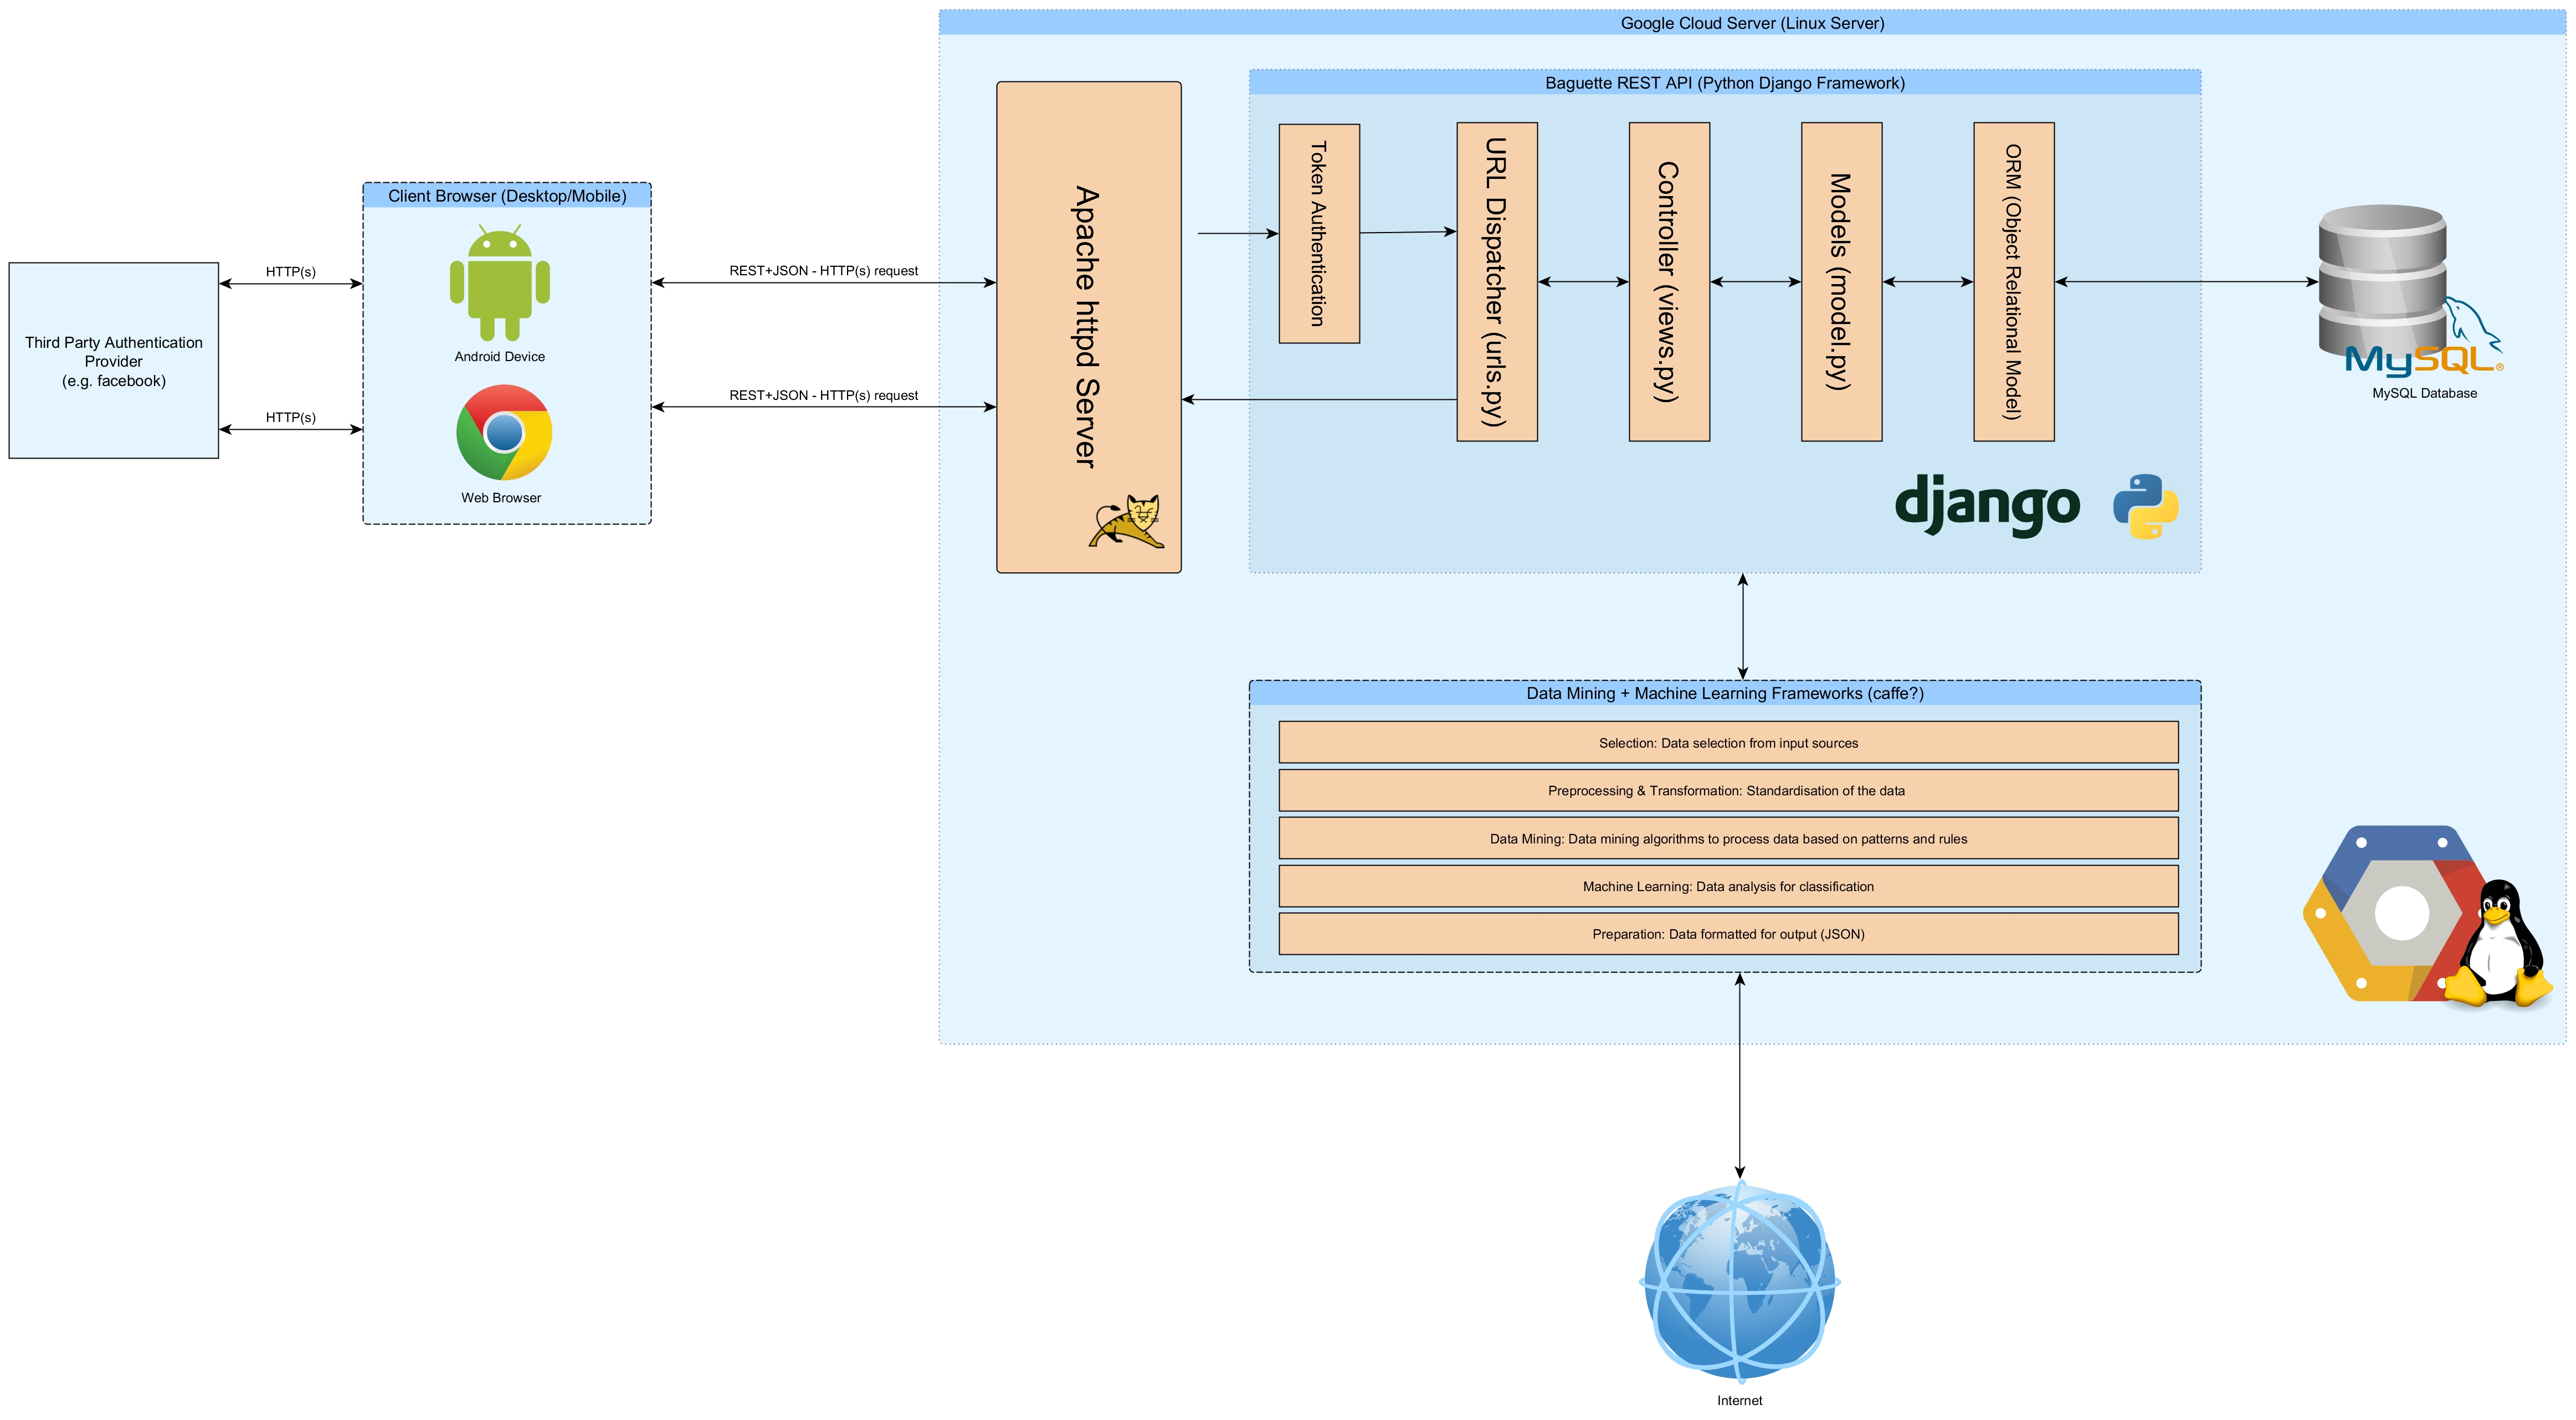
\includegraphics[width=180mm]{inc/architecture_diagram.jpg}
    \caption{derp}
    \label{fig:sentiment_analysis_step2b}
  \end{minipage}
\end{figure}

\end{landscape}
